%!TEX root = ../PhDthesis.tex
\chapter{Exploring the role of inhibition in cortical development and surround modulation}

In the previous chapter we explored the spatially calibrated SCAL
model, establishing how various sources of evidence about the spatial
structure of V1 projections relate to each other. While this model was
able to account for the size tuning properties of the visual cortex
quite well, it also exhibited two major shortcomings. Most importantly
it highlighted that a model lacking disinct excitatory and inhibitory
populations will not be able to capture the diversity in connectivity
profiles. Secondly we showed that based on the known lack of truly
long-range inhibitory projections must be mediated by a di-synaptic
mechanism mediated by long-range excitatory connectivity.

Additionally, in the literature section we described the known
properties of various inhibitory cell classes and what roles they
might perform. In particular we discovered that PV and SOM-expressing
interneurons exhibit highly distinct response properties and
layer-specific expression patterns.  With recent techniques allowing
targeting of specific populations there is now huge interest in
understanding their role both in development and in mediating and
gating the both contextual and attentional modulation phenomena.

In this chapter we will propose models that incorporate the distinct
response properties of PV and SOM interneuron populations, allowing us
to make concrete predictions about their role in developmental and
behavioural phenomena. First we establish that the fast and linear
response of the PV-ir, fast-spiking interneuron population makes them
ideally suited towards controlling feedforward activity, sparsifying
activity and thereby driving map formation. While demonstrating robust
and stable map formation even in the presence of strong lateral
excitation, we show that the broad tuning properties of the PV
population makes them badly suited to mediate context and feature
specific modulation. By introducing a secondary inhibitory population
modeled on the response properties of SOM+ neurons we extend the model
to demonstrate how their weaker and facilitating inputs
\citep{Bartley2008,Beierlein2003,Bartley2008,Tan2008} lead to the
development of highly tuned neurons, which respond only for high
contrasts or large stimuli, thereby mediating a range of surround
modulation phenomena.

\section{Methods}

\subsection{The SEPI Model}

The \textbf{S}hort-\textbf{R}ange \textbf{E}xcitation \textbf{P}V
\textbf{Inhibition} (SEPI) model is based on the same principles and
spatial profiles that were described for the SCAL model in the
previous chapter. However unlike SCAL the model has a distinct
excitatory and inhibitory V1 population, which both receive afferent
input and are connected to each other recurrently. The architecture
diagram in \ref{SEPIDiagram} shows the two sheets and projections
between them. When comparing this against the SCAL model diagram (see
\ref{SCALDiagram}), we can see that the spatial scales of the various
projections are unchanged they have simply been split up between the
populations.

\begin{figure}
	\centering
        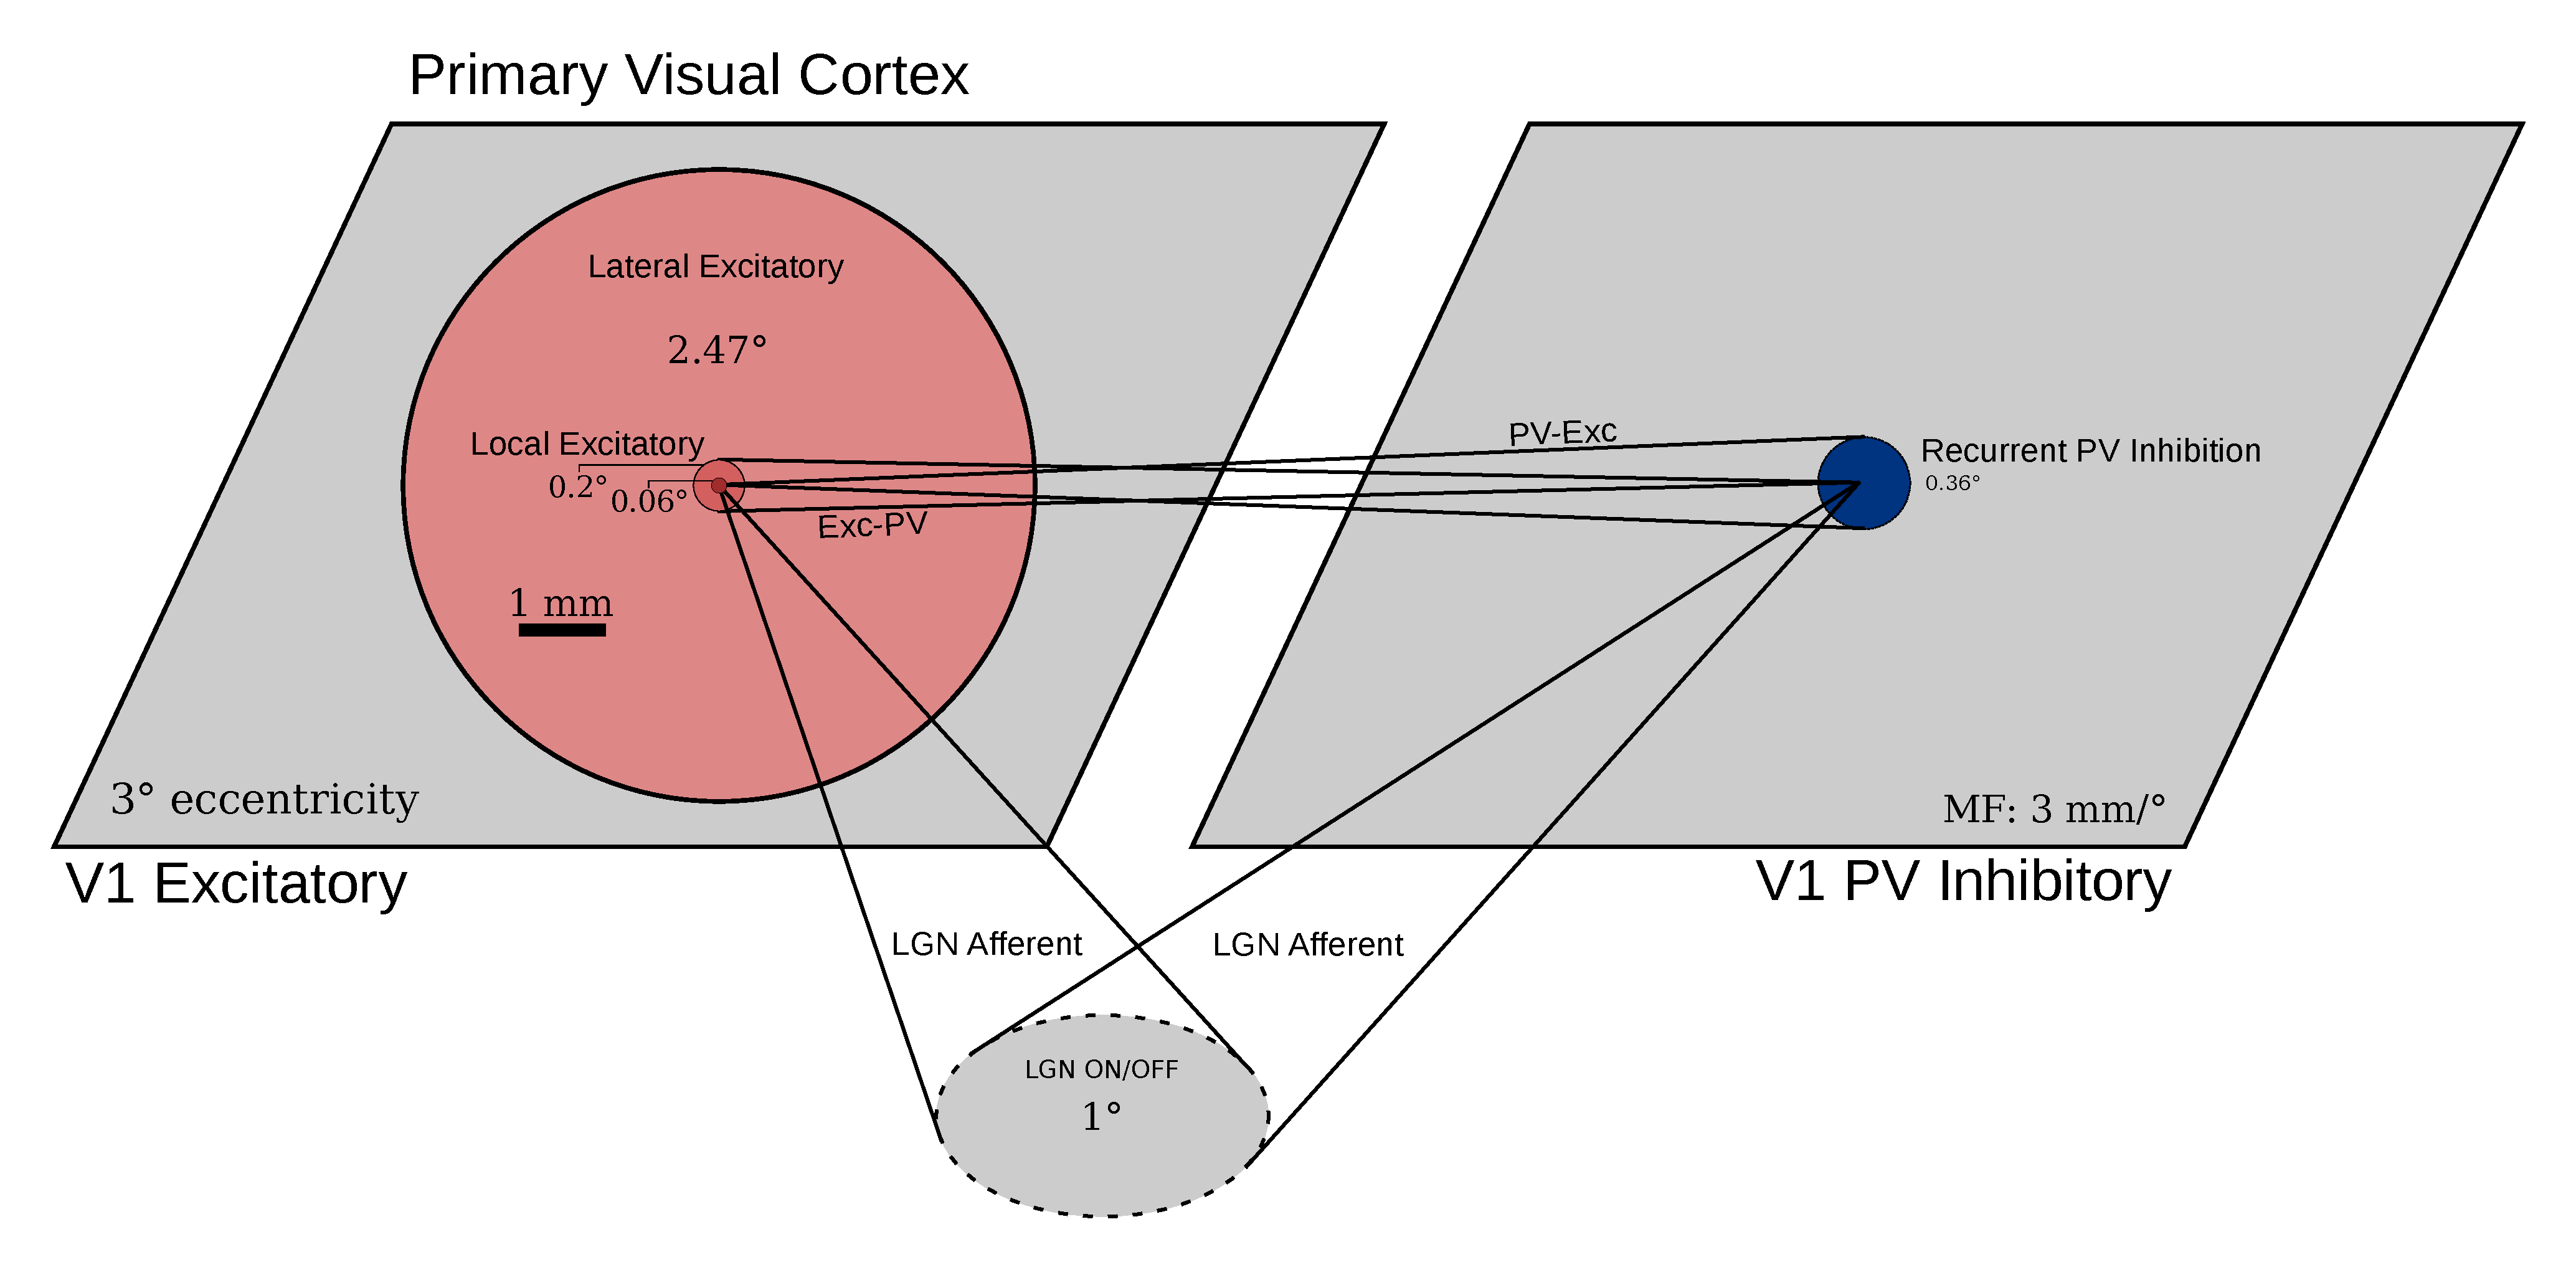
\includegraphics[width=1.0\textwidth]{SEPI_Diagram.pdf}
	\caption{Diagram of the SEPI V1 stage of the model showing the
          spatial scales of the various excitatory (red) and
          inhibitory (blue) connections. Satured colors indicate the
          kernel radii, while lightly shaded regions indicate kernel
          cut-off extents.}
	\label{SEPIDiagram}
\end{figure}

\subsection{Assessing the quality of orientation maps} \label{metrics}

A major component of the analysis applied in this section is to assess
the sensitivity of the model to changes in the response properties of
the different cell classes. Therefore we have to establish a number
metrics to assess the robustness of the model to changes in contrast
by assessing the quality of orientation map organization of the
excitatory V1 neurons map. There are a variety of measures to assess
these properties but we will focus on three in particular, smoothness,
stability and pinwheel density.

\subsubsection{Pinwheel density}

Through empirical observation that orientation maps across species
share a fundamental property, that pinwheel count in biological
orientation maps scales linearly with hypercolumn size, specifically
that there are $\pi$ orientation pinwheels within the area of one
hypercolumn, when averaging over sufficiently large cortical
areas. This dimensionless, statistical measure of pinwheel
distribution is thought to reflect a universal constant of map
organization, converging to across carnivorans, primates, cats, and
tree shrews \citep{Kaschube2010, Keil2012}. This value was predicted
by a theoretical model of map organization and has strong empirical
evidence, with a mean pinwheel density across four species (tree
shrew, galago, cat, and ferret) statistically indistinguishable from
$\pi$.

To determine the pinwheel density for any given map, the hypercolumn
distance is computed and all all pinwheel centers are found. Pinwheel
centers are located at the intersection of the zero contours of the
real and imaginary components in the polar representation of
orientation preference \citep{Lowel1998}. Then we simply divide the
number of pinwheels in the modelled area by the number of hypercolumns
to arrive at the pinwheel density.

\subsubsection{Stability}

The stability of orientation maps is determined by determing the
average orientation similarity index of the orientation map over the
course of development. To assess similarity quantitatively
\cite{Chapman1996} computed the correlation of orientation preference
at each developmental age with the organized preference map observed
in the final recording for that animal. As in \cite{Stevens2013} we
normalize these similarity values to fall between 0 (completely
uncorrelated) to 1 (identical orientation preference). The orientation
similarity index is therefore defined as:

\begin{equation}
  OSI = 1 - \frac{4}{n\pi} \sum_{i}\abs{(F_{i}-O_{i})mod(\frac{\pi}{2})}
\end{equation}

By averaging the OSI at every 1000 development steps we can
numerically compare the stability of the model over time. Note that
this does not provide a measure that is comparable across models
because this measure is heavily influenced by the speed of learning
but it does allow us to assess the effect of changing specific
parameters on the stability of the model.

\section{Results}

\subsection{Development}

The role of inhibition in development is hugely important, as
evidenced by the fact that a variety of pathological conditions have
been tied to changes in the inhibitory cell classes in the cortex
(cite). Modeling the role of these cell classes in development and
specifically a rate-based modeling requires capturing their response
properties. Since the synaptic projection develop as a result of these
properties, the tuning properties of the modeled neurons in the
developed model will let us concrete predictions about the role of
these neurons in shaping the development.

Accurately capturing the response of these neurons in a rate based
model presents a number of challenges. Additionally a lot of the data
about these cell classes comes from mouse data where the genetic
manipulation of specific cell classes has recently become possible. At
the same time this provides a great opportunity to establish whether
the response kinetics of the neurons can predict their final tuning
properties in the model and how manipulating them can affect both
development and the instantaneous response of the model to specific
stimuli.

In the literature review we identified the parvalbumin (PV) expressing
interneurons, which include fast-spiking basket and clutch cells, as
the most likely candidate to provide feedforward inhibition and
controlling the gain of the response in of the pyramidal cells. Their
high abundance in the thalamocortical recipient layer 4 and layers 2/3
making up over half the population in each \citep{VanBrederode1990} as
well as their involvement in the onset of critical period
\citep{Fagiolini2000} and effect on the columnar organization of the
visual cortex \citep{Hensch2004} makes them of particular interest. The
other defining characteristics of the PV population is their fast
response \citep{Cruikshank2007,Gabernet2005}, and their ability to
linearly match the excitation in the excitatory population
\citep{Atallah2012}. This closes matches the role of the inhibitory
projection in the SCAL model, which provides divisive gain control and
is directly coupled to the response of the excitatory population.

In order to capture the response of the PV population we apply only
half-rectification to the inhibitory population, as basket cells
generally have a very low spiking threshold \citep{Ma2011}, and the
difficulty involved in balancing homeostatic thresholds in two
populations. Secondly we keep the effect of the inhibition divisive in
their effect on both each other and on pyramidal cells. The PVir cells
provide strong peri-somatic input, which can act as shunting
inhibition and therefore behave as a divisive gain control mechanism
\citep{Atallah2012, Wilson2012}. These properties distinguish them
from the other major class of inhibitory interneurons the somatostatin
(Sst) expressing population, which receive weaker but facilitating
inputs \citep{Beierlein2003,Bartley2008,Tan2008}.

We will attempt to model this difference by exploring the effect of
changing the linearity and time constant of the response and explore
how these properties affect the development of the cortex making use
of the metrics described in \ref{metrics}.

\subsubsection{Linearity and time profile of inhibitory responses}

The linearity and time constant of the inhibitory population are two
of the major ways the activity of the two inhibitory populations can
be decoupled. The expectation here is that if the inhibitory
population responds sublinearly to afferent and recurrent input it
will either not be able to match the feedforward excitation leading to
diffuse activity with weak boundaries between columns, and therefore
weaker selectivity and stability but higher homogeneity. In contrast
supralinear responses should result in overly strong inhibition, which
will drive stronger competition, resulting in more selective and more
stable regions. How this affects the actual organization of the model
is less clear.

The results of the parameter analysis are shown in figure
\ref{SEPILinearity}, showing the effect of these parameters on a
number of metrics. This includes a measure of stability over time,
orientation selectivity, local homogeneity or smoothness and finally
the pinwheel density metric, used to assess the quality of the
maps. The immediately striking result is that narrow band of good
(near $\pi$) pinwheel density ($\rho$) in the linear region of the
response. Additionally we can see what we predicted low stability and
selectivity at low contrasts, which presumably contributes to the
large degree of homogeneity.

Additionally we also compute an assessment of the retinotopy of the
model by comparing the center-of-gravity (CoG) of feedforward
connections to the position of that neuron in the map. The CoG shift
reveals how strong inhibition regimes can disrupt retinotopy, which
leads to distortions in the orientation map, which is reflected in the
pinwheel density.

\begin{figure}
	\centering
        \includegraphics[width=1.0\textwidth]{./results/sepi/SEPI_Linearity.pdf}
	\caption{Parameter exploration to determine how the linearity and
      time constant of inhibitory responses affect development. A) A
      measure of stability of the model over time, integrating the
      similarity index of the model over time. B) Orientation
      selectivity in the model measured using orientation map
      measurements. C) The average local homogeneity index measuring
      the smoothness of the map at a particular spatial scale. D)
      Pinwheel density of the model, which should approach $\pi$ for a
      perfect map.}
	\label{SEPILinearity}
\end{figure}

Overall we can conclude that a linear response but not necessarily a
very fast response is required to drive the development of a
high-quality orientation map.

\subsubsection{Robustness to long-range excitation}

At this point two separate models have been introduced, the SCAL and
SEPI models, which are very similar differing mostly by the fact that
the latter has distinct excitatory and inhibitory populations. The
major reason why the populations were split in this way is to match
the anatomy, but does this actually buy us anything from a functional
perspective. One major other reason we introduced an inhibitory
population is to investigate the role of long-range lateral excitatory
connections in driving contextual modulation effects. However in order
for these neurons to actually have any effect they need to actually be
able to modulate neuron activity fairly strongly. Therefore assessing
how the models hold up in the presence of strong lateral excitation
under varying contrast levels is particularly interesting. Here we
will compare how the SCAL and SEPI models deal with varying levels of
contrast and lateral excitation to investigate whether separating the
populations has any benefits in addition to being more anatomically
realistic.

\begin{figure}
	\centering
        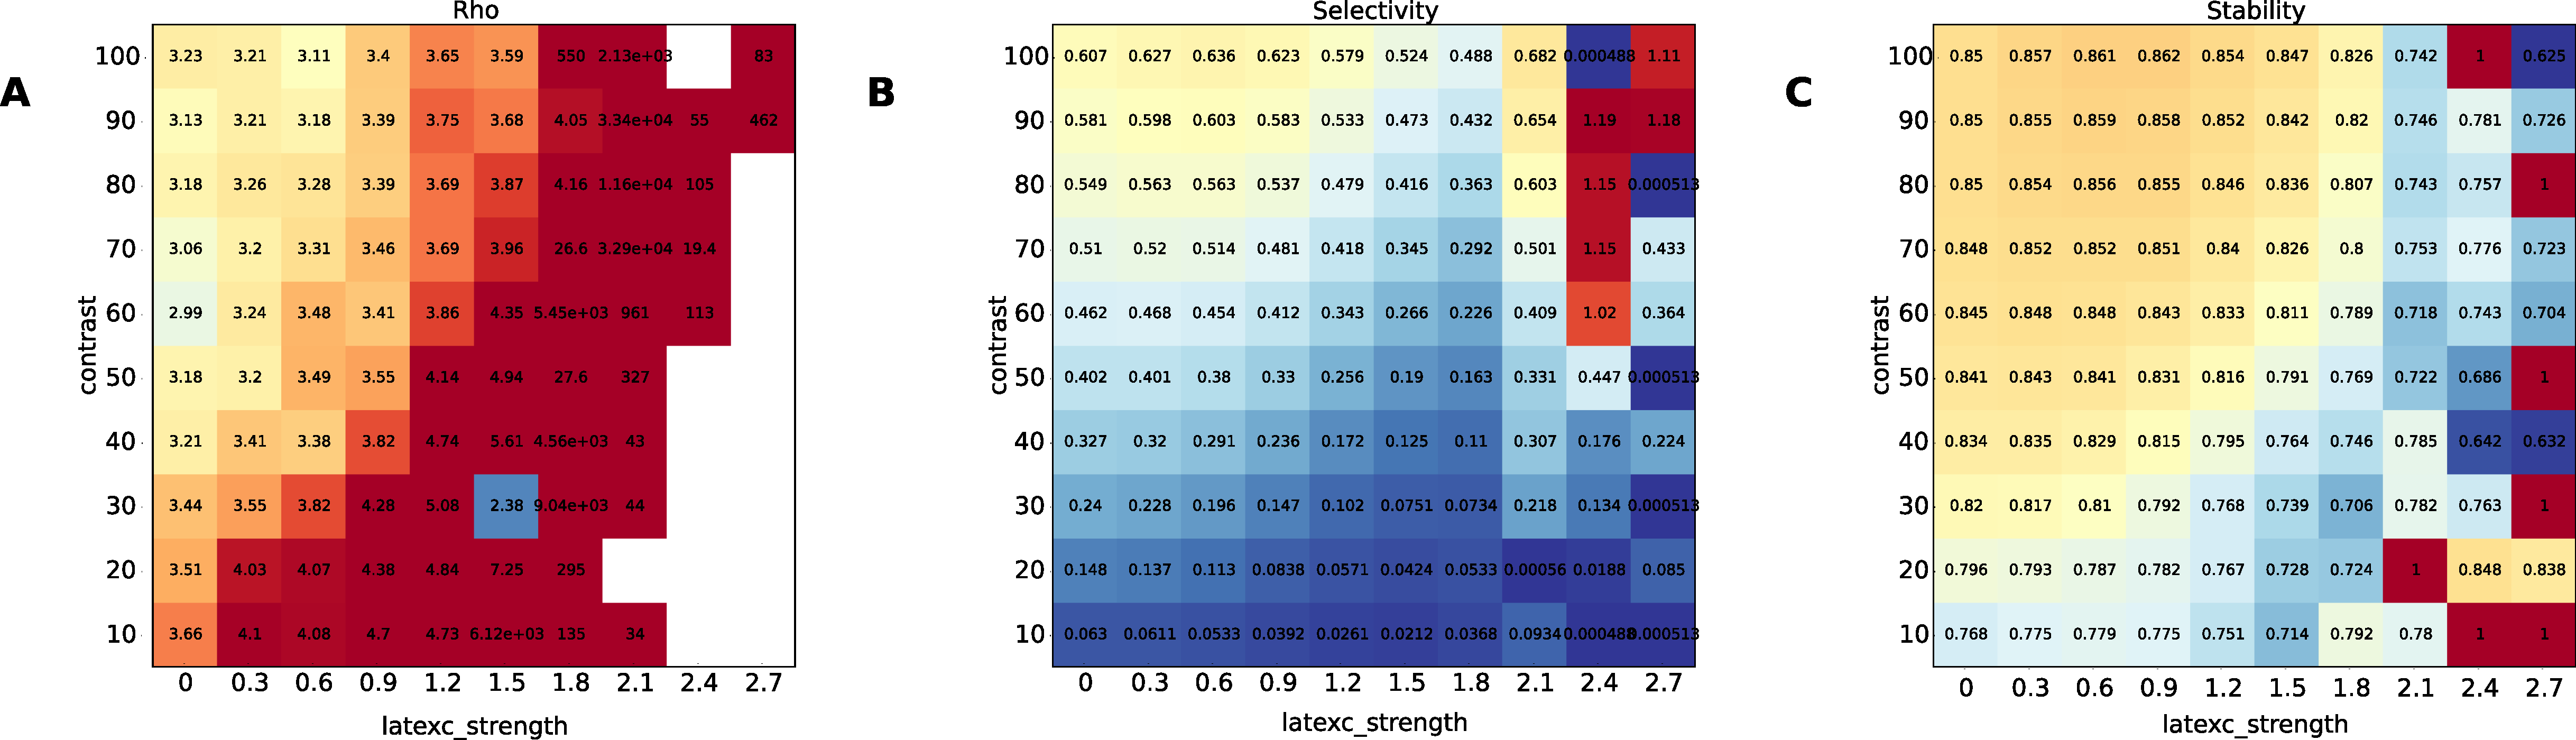
\includegraphics[width=1.0\textwidth]{SCAL_LatStability.pdf}
	\caption{Parameter explorations of three separate metrics of
          orientation map development using the SCAL model. Varied
          parameters are the strength of long-range lateral excitation
          and the stimulus contrast. The three metrics are \textbf{A}
          the $\rho$ pinwheel density metric, which characterizes the
          quality of the map, \textbf{B} the average selectivity over
          the time course of development and \textbf{C} the stability
          metric measuring how much the map changes throughout the
          course of development. The model shows good robustness to
          varying stimulus contrasts at low levels of lateral
          excitation but quickly deteriorates with increasing levels
          of excitation. White values indicate instabilities in the
          model causing the model to terminate.}
	\label{SCALStability}
\end{figure}


\begin{figure}
	\centering
        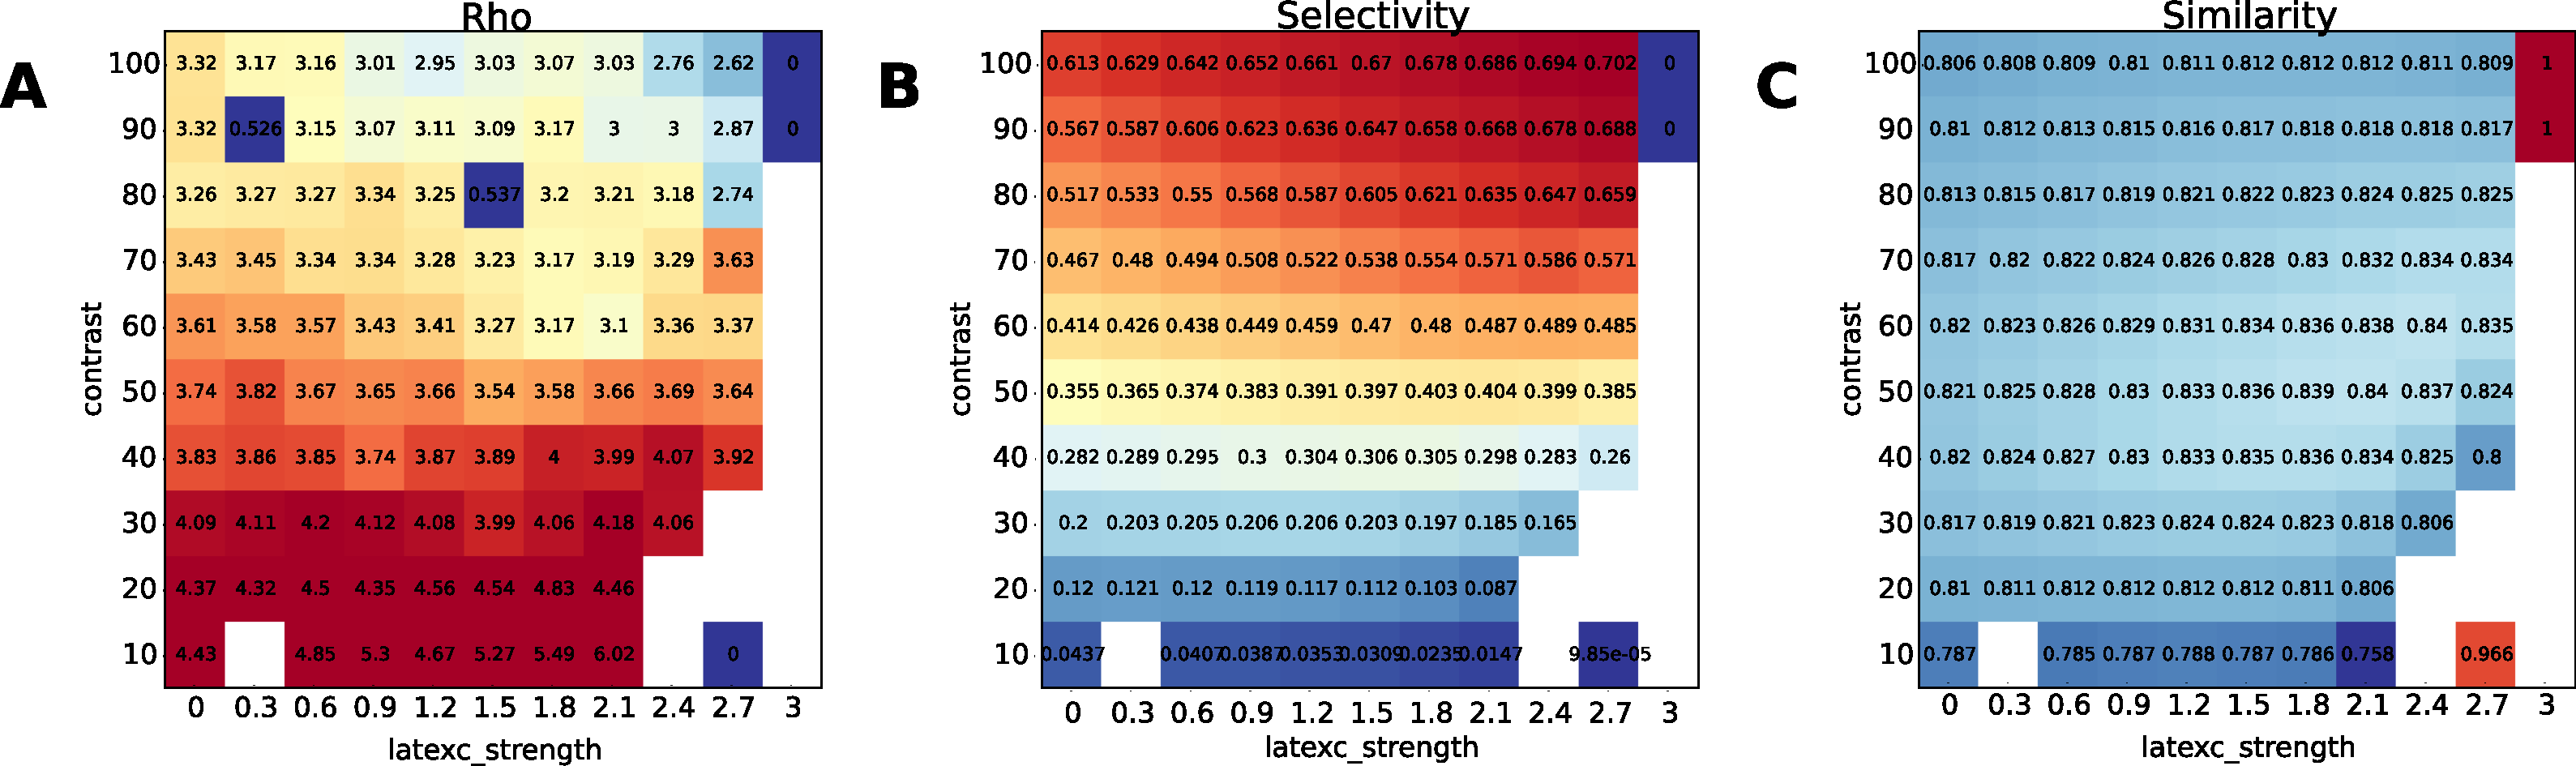
\includegraphics[width=1.0\textwidth]{SEPI_LatStability.pdf}
	\caption{Parameter explorations of three separate metrics of
          orientation map development using the SEPI model. In
          comparison to the SCAL model the pinwheel metric is not as
          robust to changes in contrast, however the model is far more
          robust to strong lateral excitation and maintains almost
          uniform stability across almost all explored parameter
          values. Uncoupling of excitation and inhibition allows the
          model to handle changes in parameter strengths but in
          absence of a homeostatic mechanism may disrupt map formation
          at low contrasts.}
	\label{SEPIStability}
\end{figure}

\section{The SEPI Model}

Exploring the effect on the SEPI and SCAL models has told us a lot
about the behavior of the models and how they develop. Before looking
at the response of these models to more complex stimuli, it is
important to confirm that the SEPI model actually does as well on the
spatial tuning characteristics we explored in the previous chapter.

In particular we are interested whether decoupling the excitatory and
inhibitory population has resulted in any increases in the diversity
of responses and changed spatial profile of their projections. Before
looking at that in more detail, the \ref{SEPIORTuning} confirms that
the model still exhibits very good map organization and even improved
contrast invariance.

\begin{figure}
	\centering
    \includegraphics[width=1.0\textwidth]{./results/sepi/SEPI_V1_ORTuning.pdf}
	\caption{SEPI model orientation tuning properties after presenting
      20,000 oriented Gaussian patterns. A) Orientation map measured
      by presenting sine gratings at the optimal spatial frequency to
      the model, along with the locations of the receptive fields
      shown in B. B) Gabor-fits to receptive fields measured using
      sparse random noise. C) Orientation tuning curve of a single
      neuron across contrasts, demonstrating largely contrast
      dependent orientation tuning.}
	\label{SEPIORTuning}
\end{figure}

Of particular interest is the effect on contrast dependent size tuning
shifts. Recall that the GCAL model showed very little contrast
dependent size tuning changes due to the inhibition being purely
subtractive. The SCAL model demonstrated a strong shift, however it
severely lacked in diversity. As can be seen in \ref{SEPI_DoG_Contrast},
introducing separate populations has resulted in far greater diversity
and a shift that matches experimental results in its magnitude,
i.e. by separating the populations we have achieved a considerably
improved fit to the experimental data.

\begin{figure}
	\centering
        \includegraphics[width=0.8\textwidth]{./results/sepi/SEPI_V1_DoG_Contrast.pdf}
	\caption{Contrast dependent shifts in size tuning as estimated by
      the DoG model. A) Spatial constant of the excitatory center of
      the DoG model at low vs. high contrast. B) Distribution of
      contrast dependent shifts, showing a much better match to the
      experimental data than GCAL or SCAL (see \ref{ContrastShift}.}
	\label{SEPI_DoG_Contrast}
\end{figure}

Introducing a separate inhibitory population also allows us to compare
the spatial and orientation profile of inhibitory neurons more
realistically since they no longer reflect the activation of the joint
excitatory/inhibitory population. When comparing
\ref{SEPI_OR_Distributions} we can see that the neurons are no longer
as strongly biased toward the preferred orientation of the excitatory
neuron, this is a direct result of much broader orientation tuning in
the inhibitory PV population.

\begin{figure}
	\centering
        \includegraphics[width=1.0\textwidth]{./results/sepi/SEPI_Inh_OR_Distributions.pdf}
	\caption{Spatial distribution of weights targetting A)
      iso-orientation regions, B) oblique-orientation regions and C)
      cross-orientation regions.}
	\label{SEPI_OR_Distributions}
\end{figure}

Finally we can confirm the spatial and orientation tuning properties
of the SEPI model in another way. By computing the local homogeneity
index we can compute the smoothness of the map at a specific spatial
scale. In the original study \citep{Nauhaus2008} the spatial constant
used was $200 \mu m$, which is approximately the size of the dendritic
integration area. By setting an equivalent $\sigma$ we can once again
confirm whether the rough spatial scale of the map matches what we
know about the monkey cortex. By plotting the LHI vs the orientation
tuning width, shown in \ref{SEPILHI}, we can observe that the model
indeed matches the macaque very closely.

\begin{figure}
	\centering
        \includegraphics[width=0.8\textwidth]{./results/sepi/SEPI_LHI.pdf}
	\caption{Local homogeneity index against tuning width in the SEPI
      model compared to experimental results from monkey and
      macaque. Reproduced from \cite{Nauhaus2008}.}
	\label{SEPILHI}
\end{figure}


\section{Discussion}

In this chapter we have explored how distinct excitatory and
inhibitory modeled after the pyramidal and basket cells in the visual
cortex interact to give rise to robust and stable map formation.

\subsection{On the role of Parvalbumin expressing neurons in the cortex}

\subsection{On long-range contextual effects}
